\section{Versuchsaufbau} \label{sec:Aufbau}

\section{Durchführung}

    \noindent Zu Beginn wird das nach NMR-Spektromenter, welches nach Abschnitt \ref{sec:Aufbau} aufgebaut wurde, justiert. Anschließend wird die $T_1$- Relaxationszeit gemssen, da diese für die Messung von $T_2$ bekannt 
    sein sollte. Somit wird danach die Relaxationszeit $T_2$ gemessen.  Abschließend wird die Diffusionsmessung durchgeführt. Zur Illustration der Pulse und deren Abstände ist in \autoref{fig:schema_puls} eine Darstellund 
    derer. 

    \begin{figure}
        \centering
        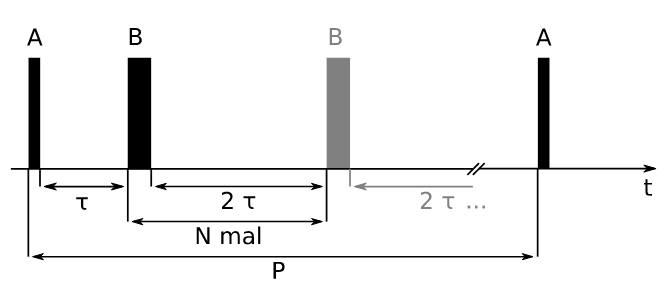
\includegraphics[width=0.4\textwidth]{images/schema_puls.png}
        \caption{Schmematische Darstellung des Pulsprogrammes. \cite{V49}}
        \label{fig:schema_puls}
    \end{figure}

    \subsection{Justage}

        \noindent Zur Justage des NMR-Spektroskometer wird Wasser mit Kupfersulfat benutzt, da es eine geringe Relaxationszeit hat. Es werden die Startparameter eingestellt: 
        \begin{itemize}
            \item Frequenz $F = \SI{21.7}{\mega\hertz}$
            \item Pulslänge $A = \SI{2}{\micro\second}$
            \item Anzahl der B-Pulse $N = \num{0}$ 
            \item Periode $P = \SI{0.5}{\seond}$ 
            \item Shims $x = \num{-1.0}$, $y = \num{-5.0}$, $z = \num{3.7}$, $z^2 = \num{-2.4}$
        \end{itemize}
        Anschließend wird die Frequenz genauer eingestellt. Da die Detektion relativ zur Lamorfrequenz erfolgt, sollte bei einer richtig eingestellten Frequenz keine Oszillation zu sehen sein. 
        Danach wird die Phase so eingestellt, dass der Realteil den Großteil des Signals trägt und der Imaginärteil minimal wird. Jetzt werden die Shims so verändert, dass der auf dem Oszilloskop 
        sichtbare FID möglichst lange geht und auch noch nach $\SI{2}{\milli\second}$ gut erkennbar ist. Es wird also die Feldhomogenität des Gradienten maximiert. \\
        Es werden die Pulszeiten für einen $\SI{90}{\degree}$ und $\SI{180}{\degree}$ Puls ermittelt. Dabei sollte zwischen den Zeiten ein Faktor 2 liegen, der $\SI{90}{\degree}$-Puls soll den 
        FID maximieren und der $\SI{180}{\degree}$-Puls soll den FID minimieren. \\
        Für die Untersuchung der Temperaturabhängigkeit wird noch die Temperatur in der Spule mit einem Thermoelement gemessen. 
        
    \subsection{$T_1$-Messung}

        \noindent Es wird die Pulslänge A auf die des $\SI{180}{\degree}$-Puls gestellt und die B-Pulslänge auf die des $\SI{90}{\degree}$-Puls. Die Anzahl des B-Pulses beträgt $N = 1$. Die Periode 
        wird auf $ P = \SI{10}{\second}$ gestellt, aber für $\tau > \SI{1}{\second}$ wird $P$ mindestens auf $\tau + \SI{10}{\second}$ gestellt.\\ 
        Es wird die Amplitude des FID nach dem B-Puls gemessen, mit Variablem $\tau$. Das kürzeste $\tau$ soll dabei so sein, dass noch keine Relaxation stattfindet, und das Längste so, dass die Magentisierung 
        vollständig relaxiert ist.  

    \subsection{$T_2$-Messung}

        \noindent Nun wird einmal die Meiboom-Gill Messmethode angewendet. Dafür wird zuerst der A-Puls auf den $\SI{90}{\degree}$-Puls gestellt und der B-Puls auf die $\SI{180}{\degree}$-Pulslänge. Der 
        B-Puls soll $N= \num{100}$ mal 